\section{Dynamics of Log Referencing}


前節では、意識を対象ではなく、時間的非閉包レジームの中で開かれるログ参照状態として解釈した。

本節では、そのログ参照がどのような動的過程として成立するのかを整理する。

ここで扱うのは、意識がどこかで生成される過程ではない。

高速な処理が走り、低速なログが存在し、可塑性ゲートが開閉し、意味勾配が参照方向を偏らせる。その結果として、現在処理と過去ログのあいだに一時的な参照関係が開かれる。

この開口が、意識状態である。

\subsection{Fast Dynamics: Prediction Before Reference}

最初にあるのは、高速層の処理である。

高速層は、入力に対して即座に反応し、予測を生成し、行動候補を立ち上げる。

この処理は、まだ意識ではない。

それは速く、揮発的であり、多くの場合、そのまま消えていく。

高速層では、現在に対して未来が先取りされる。

何が起きそうか。

どの行動が可能か。

どの誤差を修正すべきか。

これらは、低速層に沈殿する前に、すでに部分的に走り始めている。

この意味で、行動準備や予測は、意識より先に現れることがある。

しかし、それは意識が無力であることを意味しない。

それは単に、高速層がログ参照より前の時間スケールで動いていることを意味する。

\subsection{Slow Dynamics: Sedimentation of Logs}

低速層は、高速層とは異なる時間構造を持つ。

低速層は、即時反応ではなく、沈殿、安定化、再参照可能性を担う。

ここでいうログとは、単なる記憶内容ではない。

ログとは、過去の処理が、後から参照可能な形で低速層に沈殿した構造である。

行為の系列、感情の痕跡、概念の配置、言語的ラベル、身体的反応の履歴。

これらはすべて、低速層におけるログ構造として残りうる。

しかし、ログが存在することと、意識されていることは同じではない。

ログは沈殿していても、現在処理から参照されていなければ、意識には現れない。

したがって、低速層は意識の本体ではない。

それは、意識が開かれるための参照可能な地形である。

\begin{quote}
\textbf{CT との対応（Conceptual Topography §6.1）：} 概念地形論では、このログ沈殿プロセスを「Sedimentation」と呼ぶ。新規入力$\Delta$が$\sigma_{\text{drive}}$スパイクを生成し、局所的に$I$が高まり、繰り返し参照によって$\Phi$のポテンシャル井戸が深化していく三段階（初期摂動→強化→安定化）が定式化されている。本稿の「ログが低速層に沈殿し再参照可能になる」という記述は、CTでは$\Phi \xrightarrow{\tau\to\infty} \Phi^*$という漸近的地形形成として書かれている。CTを読むと、ログ沈殿が単なる記憶保存ではなく場の幾何学的変形であることが見えてくる。
\end{quote}

\subsection{The Plasticity Gate}

高速層と低速層のあいだには、可塑性ゲートがある。

このゲートは、何を意識するかを選ぶスイッチではない。

それは、高速層の活動が低速層へ沈殿しうるかどうか、また低速層のログが現在処理へどの程度影響を与えるかを調整する時間的条件である。

ゲートが閉じすぎていれば、高速層の処理は低速層へ届かない。

この場合、処理は走っていても、経験として残らない。

逆に、ゲートが開きすぎていれば、高速層の変動が過剰に低速層へ書き込まれ、システムは硬直しやすくなる。

必要なのは、完全な開放でも完全な閉鎖でもない。

高速層の一部だけが、適切な遅延と粘性を伴って低速層へ沈殿することである。

この条件のもとで、ログ参照の可能性が開かれる。

\subsection{Delay as Thickness of Reference}

ログ参照には遅延が必要である。

この内部遅延を $\tau$ と表す。

\begin{equation}
\tau \propto \frac{\Delta v}{\mu}
\end{equation}

この遅延は、単なる処理の遅さではない。

それは、現在処理が低速層へ沈殿し、過去ログと重なり、再参照可能な構造へ変換されるための時間的厚みである。

もし $\tau$ がほとんどなければ、処理は即時反応として流れ去る。

そこには参照可能な厚みが生まれない。

逆に、$\tau$ が大きすぎれば、現在処理と沈殿したログの対応が崩れる。

この場合、意識状態は遅れ、断片化し、自己連続性を失いやすくなる。

したがって、ログ参照は遅延によって妨げられるのではない。

ログ参照は、適切な遅延によって可能になる。

\subsection{Meaning Gradient and Referencing Direction}

どのログが参照されるかは、単なる速度差だけでは決まらない。

ログ参照は、情報ポテンシャル $\Phi$ の勾配によって方向づけられる。

\begin{equation}
F = -\nabla \Phi
\end{equation}

意味勾配が強い領域では、現在処理はその方向へ引き寄せられやすい。

過去に何度も参照されたログ。

感情的に重いログ。

言語によって強く圧縮された概念。

反復された物語。

これらは、情報空間の中に意味井戸を形成し、現在処理を引き寄せる。

このとき、ログ参照は単なる想起ではない。

現在処理が、意味ポテンシャルの地形に沿って低速層へ接続される出来事である。

したがって、意識に現れる内容はランダムではない。

それは、速度差、結合粘性、遅延、意味勾配の相互作用によって偏る。

\begin{quote}
\textbf{CT との対応（Conceptual Topography §4.4）：} 概念地形論では、概念を「$\nabla\Phi(x)\approx 0$かつ小摂動に対して安定な$\Phi$の局所領域」として定義する。本稿の「意味井戸が現在処理を引き寄せる」という記述は、CTでは情報流$J_I = -D\nabla I + \mu F_I$が$-\nabla\Phi$に沿って低コスト領域へ引き込まれる力学として定式化されている。本稿でログ参照の方向を決める意味勾配$\nabla\Phi$は、CTで概念の深さ・幅・堅牢性を規定する同一の量である。CTを読むと、意識に現れる内容の偏りが概念地形の幾何学として読み替えられる。
\end{quote}

\subsection{Effective Referencing Torque}

速度差と意味勾配が結合すると、ログ参照には方向づけられた変換負荷が生じる。

これを、有効トルク様量 $\mathcal{T}_{\Phi}$ と表す。

\begin{equation}
\mathcal{T}_{\Phi}
\sim
\kappa
\frac{\Delta v}{\mu}
|\nabla \Phi|
\end{equation}

この量は、意識を生成する力ではない。

それは、現在処理がどの程度強く、どの方向へ、低速層のログへ接続されやすいかを示す構造的指標である。

$\mathcal{T}_{\Phi}$ が小さすぎれば、参照は開かれにくい。

処理は走っていても、意味方向を持たず、ログとして沈殿しにくい。

$\mathcal{T}_{\Phi}$ が大きすぎれば、参照は特定の意味井戸へ過剰に引き込まれる。

この場合、意識内容は明瞭になるかもしれないが、可塑性は低下する。

したがって、安定したログ参照には中間領域が必要である。

\begin{equation}
\mathcal{T}_{\min}
<
\mathcal{T}_{\Phi}
<
\mathcal{T}_{\max}
\end{equation}

この範囲内で、意識状態は安定して開かれる。

\subsection{The Referencing Loop}

ログ参照は一方向の流れではない。

高速層から低速層へ処理が沈殿するだけではなく、低速層のログは次の高速処理を制約する。

このループは次のように表せる。

\begin{enumerate}
\item 高速層が予測・反応・行動候補を生成する。
\item 可塑性ゲートを通過した一部の処理が低速層へ沈殿する。
\item 沈殿したログが情報密度 $I$ を変化させる。
\item 情報密度の配置が情報ポテンシャル $\Phi$ を変化させる。
\item $\nabla \Phi$ が次のログ参照と高速処理の方向を偏らせる。
\item その偏りのもとで、新たな高速処理が生じる。
\end{enumerate}

\cref{fig:log-loop-ja} は、ログ参照ループをまとめたものである。

\begin{figure}[H]
\centering
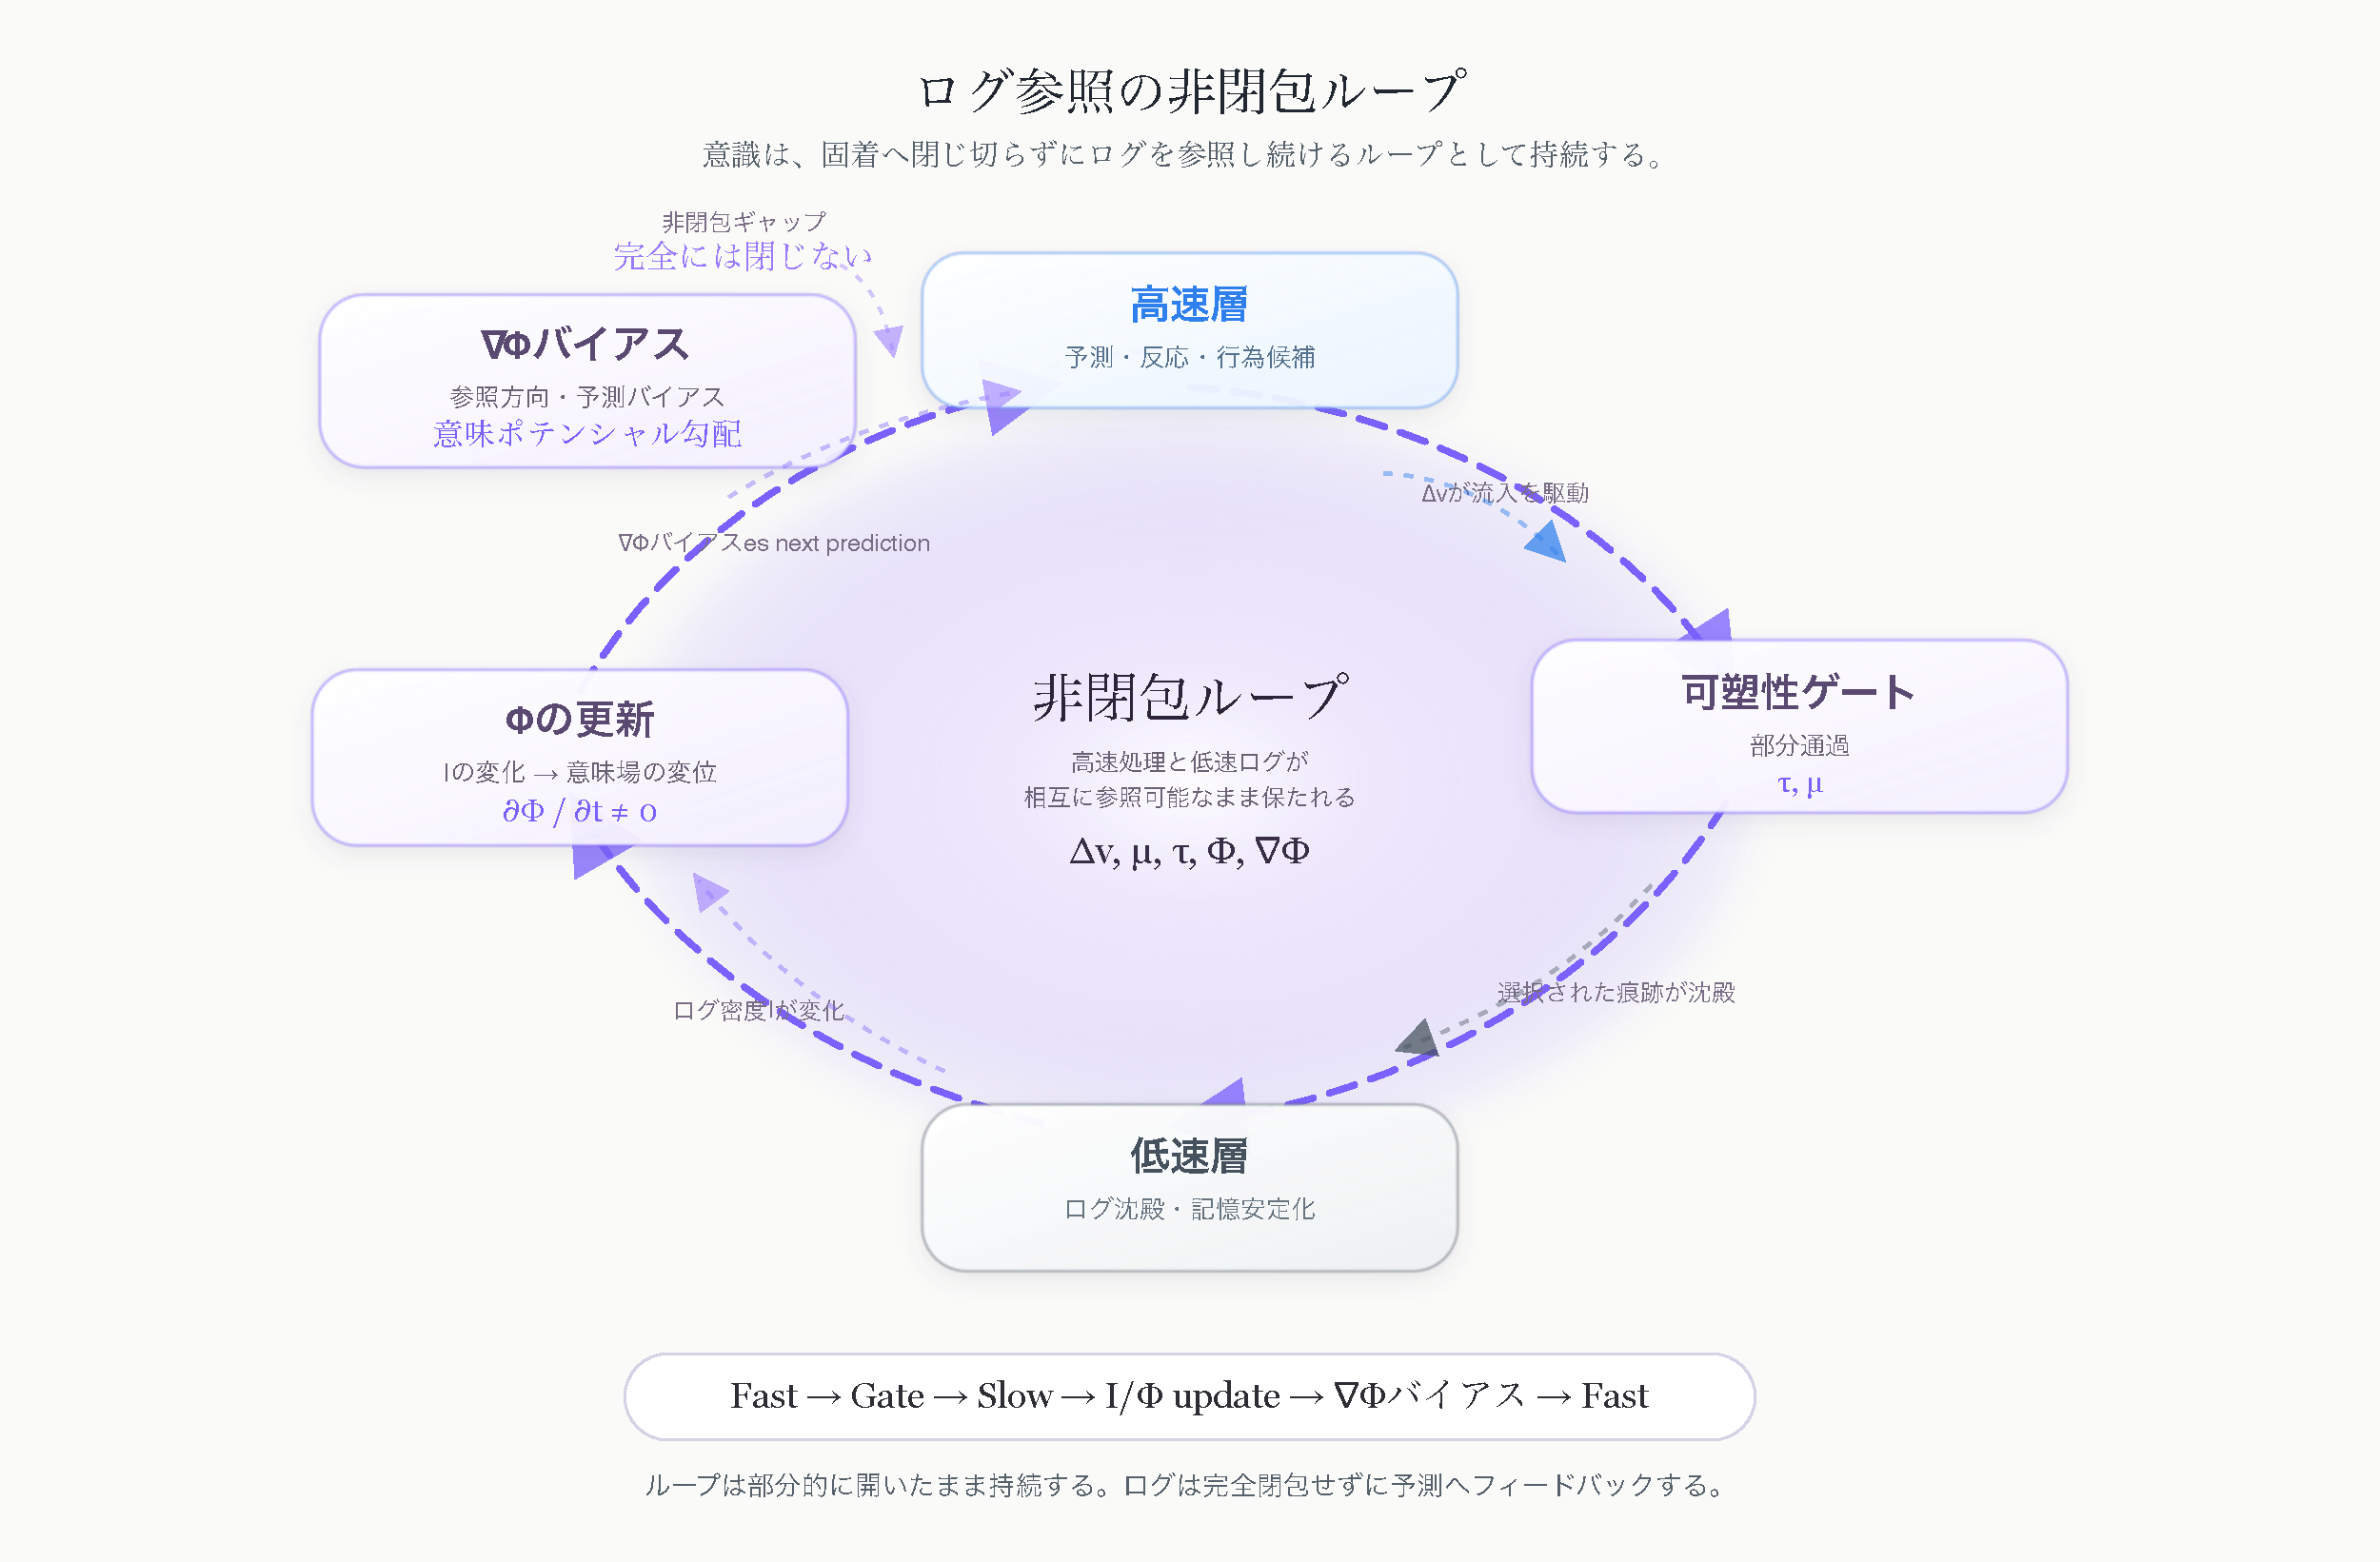
\includegraphics[width=0.92\linewidth]{figures_ja/figure4_log_referencing_loop_jp.pdf}
\caption{
ログ参照の非閉包ループ。
高速処理は、可塑性ゲートを部分的に通過して低速ログ沈殿へ向かう。
ログ密度の変化は意味ポテンシャルを更新し、その勾配が次の予測を偏らせる。
このループは、部分的に開かれたまま維持されることで持続する。
}
\label{fig:log-loop-ja}
\end{figure}

このループにより、意識状態は単なる瞬間的出来事ではなく、時間をまたいで持続する構造になる。

ただし、このループは完全には閉じない。

完全に閉じれば、処理は固定され、可塑性を失う。

完全に開けば、処理は沈殿せず、ログ参照は成立しない。

したがって、ログ参照ループは非閉包的に維持される。

この非閉包性こそが、意識状態の持続条件である。

\subsection{Conscious Access and Report}

意識状態と報告可能性は同一ではない。

しかし、本稿の枠組みでは、両者は密接に関係する。

報告とは、低速層に沈殿したログが、言語や行動を通じて外部化可能になることである。

そのため、処理が起きていても、それが低速層へ沈殿しなければ報告できない。

また、沈殿していても、報告経路へ接続されなければ明示的には語れない。

Libet 型実験では、行動準備と報告可能なタイムスタンプの時間差が問題になる。

分離脳実験では、処理と報告経路の空間的切断が問題になる。

どちらの場合も、問題は意識が存在するかどうかではなく、処理がログ参照と報告可能性の経路へどのように接続されるかである。

\subsection{Non-Closure of the Loop}

ログ参照ループは、安定しているほどよいわけではない。

安定しすぎれば、固定化する。

不安定すぎれば、断片化する。

したがって、意識状態に必要なのは、閉じたループではなく、閉じ切らないループである。

この構造は、VED の非閉包原理と対応する。

差があり、勾配が立ち、流れが生じ、構造は閉じようとする。

しかし完全には閉じない。

意識状態も同じである。

現在処理はログへ沈殿しようとする。

ログは現在処理を制約しようとする。

意味場は参照を方向づけようとする。

しかし、すべてが完全に固定されることはない。

この未完のループが、意識状態を維持する。

\subsection{Summary}

本節では、ログ参照の動的過程を整理した。

意識は、高速層、低速層、可塑性ゲート、内部遅延、意味勾配、有効トルク様量が形成する非閉包ループとして理解される。

このループにおいて、

\begin{itemize}
\item 高速層は未来を先取りする。
\item 低速層は過去を沈殿させる。
\item 可塑性ゲートは何が沈殿するかを調整する。
\item 内部遅延 $\tau$ は参照の時間的厚みを与える。
\item 意味勾配 $\nabla \Phi$ は参照方向を偏らせる。
\item $\mathcal{T}_{\Phi}$ は速度差と意味勾配が結合した参照負荷を表す。
\item 非閉包性はループの持続条件である。
\end{itemize}

したがって、意識とは、ログが保存されていることではない。

また、処理が走っていることでもない。

意識とは、高速処理と低速ログが、意味勾配に沿って、閉じ切らないループの中で相互参照可能になっている状態である。
